\documentclass[10pt,conference,compsoc]{IEEEtran}
\usepackage{algorithm}
\usepackage{booktabs}
\usepackage{textcomp}
\usepackage{xcolor}
\usepackage[OT1]{fontenc}
\usepackage{algorithmicx} 
\usepackage{caption}
\usepackage{amsmath}
\usepackage{cite}
\usepackage{url}
\usepackage{graphicx}
\usepackage{subfigure}
\usepackage{algpseudocode}  


\def\BibTeX{{\rm B\kern-.05em{\sc i\kern-.025em b}\kern-.08em
		T\kern-.1667em\lower.7ex\hbox{E}\kern-.125emX}}
\begin{document}

	\title{GRAPHICS RENDERING BASED ON BIDIRECTIONAL REFLECTANCE\\
	{\footnotesize \textsuperscript{}Midterm Report}
	}
	
	\author{\IEEEauthorblockN{Kai WANG}
	\textit{11612909@mail.sustc.edu.cn}
	\and
	\IEEEauthorblockN{Lida ZHAO}
	\textit{11611803@mail.sustc.edu.cn}
	\and
	\IEEEauthorblockN{Zhiyuan WANG}
	\textit{11610634@mail.sustc.edu.cn}
	}
	\maketitle
	\begin{abstract}
		 During this stage, we find a more reasonable program structure. The origin code can slowly render a scene with only cubes and balls in it.  After understanding the code's fundamental structure and core functions, we add triangle into it and speed it up by modifying it to a parallel program. We also learned how to use Monte Carlo method to compute the integrating which is used in de-noising.
	\end{abstract}

	\begin{IEEEkeywords}
		Rendering, Ray Tracing, Ray-Triangle
	\end{IEEEkeywords}
	
	\section{Program structure introduction}
	We found a more reasonable program structure \cite{oneweekend} as shown in Figure 1, which helps us easily test new features or algorithms. Now we will introduce this structure and show how it works to you.
	
	All hitable objects are related to \textit{hitable} and \textit{material} classes. The  \textit{hitable} class includes location information and material type. Every \textit{hitable} instance needs to overide function \textit{hit()} which can  calculate if the given ray hit. The  \textit{material} class defines a kind of material by two functions, \textit{scatter()} and \textit{emitted()}. The function \textit{scatter()} determines if the ray is refracted or reflected and what the new ray should be. The function \textit{emitted()} determines the color change.
	
	After initialization of the model world and camera, we do shader procedure for every pixel. We firstly generate a ray from the camera and call the shader function for it. In the shader function, we check whether it hits any hittable objects in the initialed world. If so, we will call the scatter function of the hitten object. If the ray was refracted or reflected, we will iterate into the next depth coloring process. Otherwise, the shader returns all color information from function \textit{emitted()}.
	
	As a result, we obtained \textit{numberof\_samples} samples of RGB data for each pixel. We use the average as the RGB value of the pixel
	
	\begin{figure}[ht]
		\centering
		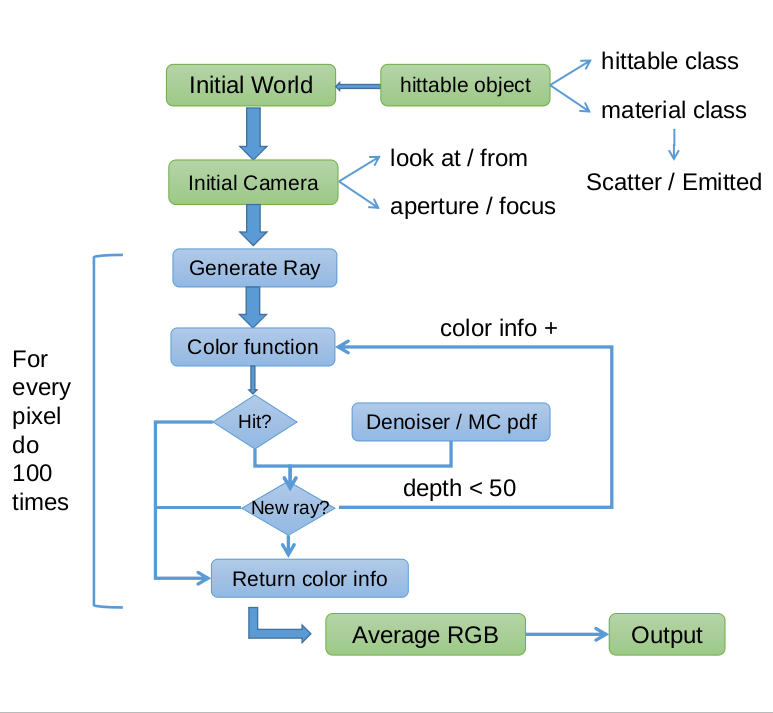
\includegraphics[scale=0.3]{./pic/structure.png}
		\caption{Program structure }
		\label{fig:label}
	\end{figure}
	\section{Triangle model}
	So far we have built sphere and rectangular models. But that is not enough because we know triangle or quadrilateral is the most basic modeling model. In fact, the triangle is more popular because it can be thought of as a two-dimensional graph, so it can save a lot of computing resources. By the way, a quadrilateral can also be substituted by two triangles.
	
	In the last section, we have introduced the \textit{hitable} class. Every hittable model needs to extend this class and implement two functions:  \textit{hit()} and \textit{bounding\_box())}. The \textit {hit()} function is used to determine if it is hit by a given ray and provides a vector p from the origin to the hit point and a normal vector from the hit point to the outside of the model. The  \textit {bounding\_box()} function is to find a minimum standard box which can surround the model.
	
	\subsection{bounding\_box function}
	This function is designed to reduce the waste of double computing by checking if the given ray hits the border\_box first. It will provide a standard box parallel to the coordinate axis. So for the triangle model, it is easy to implement. We only need to find minimum and maximum values in three dimensions separately.
	
	\subsection{hit function}	
	There are lots of algorithms for computing ray-triangle intersections. We choose to use the form that uses barycentric coordinates for the parametric plane containing the triangle because it requires no long-term storage other than the vertices of the triangle \cite{snyder1987ray}
	
	\begin{figure}[H]
		\centering
		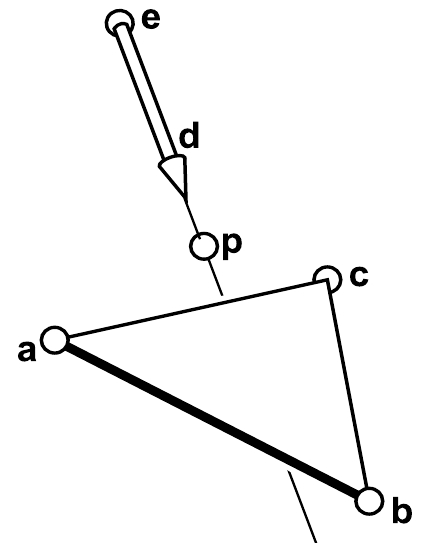
\includegraphics[scale=0.3]{./pic/ray_triangle_intersection.png}
		\caption{Ray triangle intersection}
		\label{fig:label}
	\end{figure}

	\textbf{e} is a vector points to orgin. \textbf{d} is a unit vector on ray's direction. \textbf{p} is a vector points to hit point. \textbf{a},\textbf{b} and \textbf{c} are three vertex vectors.  From intersection theory, we know hit will happen when:
	$$\textbf{e} + t\textbf{b}  = \textbf{a} + \beta\textbf{(b-a)} + \gamma\textbf{(c-a)}$$
	And hit point is in the triangle when $\beta > 0$ , $\gamma > 0$ and $\beta + \gamma < 1$. Otherwise, it will hit on outside of the triangle. It is hard to sovle $t,\beta,\gamma$. We expand vectors in fomular first.
	\begin{equation}       %开始数学环境
	\left[                %左括号
	\begin{array}{ccc}   %该矩阵一共3列,每一列都居中放置
	x_a - x_b & x_a - x_c & x_d \\
	y_a - y_b & y_a - y_c & y_d \\
	z_a - z_b & z_a -z_c & z_d
	\end{array}
	\right]                 %右括号
	\left[                %左括号
	\begin{array}{c}   %该矩阵一共3列,每一列都居中放置
	\beta\\
	\gamma\\
	t
	\end{array}
	\right]  
	=
	\left[            %左括号
	\begin{array}{c}   %该矩阵一共3列,每一列都居中放置
	x_a - x_e\\
	y_a - y_e\\
	z_a - z_e
	\end{array}
	\right] 
	\end{equation}

	The fastest classic method to solve this 3 × 3 linear system is \textit{Cramer’s rule}. This gives us the solutions. Every 3 × 3 linear system can be represented by every 3 × 3 linear system can be represented by these characters.
	\begin{equation}       %开始数学环境
	\left[                %左括号
	\begin{array}{ccc}   %该矩阵一共3列,每一列都居中放置
	a & d & g \\
	b & e & h \\
	c & f & i
	\end{array}
	\right]                 %右括号
	\left[                %左括号
	\begin{array}{c}   %该矩阵一共3列,每一列都居中放置
	\beta\\
	\gamma\\
	t
	\end{array}
	\right]  
	=
	\left[            %左括号
	\begin{array}{c}   %该矩阵一共3列,每一列都居中放置
	j\\
	k\\
	l
	\end{array}
	\right] 
	\end{equation}
	Cramer’s rule gives us :
	$$\beta = \frac{j(ei-hf)+k(gf-di)+l(dh-eg)}{M}$$
	$$\gamma = \frac{i(ak-jb) + h(jc-al) + g(bl-kc)}{M}$$
	$$t = - \frac{f(ak-jd) + e(jc-al) + d(bl - kc)}{M}$$
	$$M = a(ei-hf) + b(gf - di) + c(dh - eg)$$
	So far, we can calculate the intersection in a short time.
	\subsection{Judging the front and back}
	In the actual triangulation modeling scenario, we want the triangle to have front and back so that we can distinguish the outside and inside of the model. Because of properties like reflection, refraction, we only want it to work on the outer surface of the model.
	The algorithm we choose is to use normal vector. When we modeled, we defined the three vertices of the triangle in clockwise order from the outside perspective. When a ray comes, we compare directions of ray and triangle's normal. If the $tag$ is positive, it means that the ray hits the front of the triangle. Otherwise, it is the opposite side of the triangle.
	$$tag = p_{ray} \cdot (p_{AB}  \times {p_{BC}})$$
	
	\begin{figure}[ht]
		\centering
		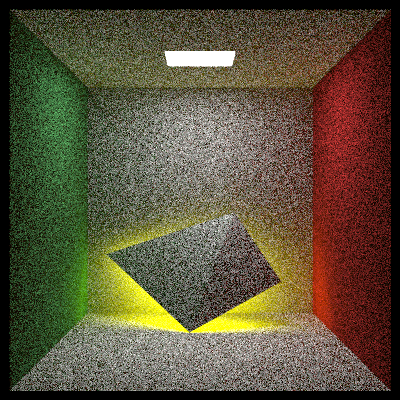
\includegraphics[scale=0.3]{./pic/triangle_sample.png}
		\caption{Triangle example}
		\label{fig:label}
	\end{figure}

\section{Noise reduction}
Now, we face a contradiction: a large number of samples will cost so much time, and the low number of samples will cause low rendering quality. So we need a way to balance them and find some way to optimize them.

\subsection{How does the noise produce?}
When we do the rendering, if the ray hit on an object with rough material, it will reflect a ray with random direction, this will produce a problem. In reality, the light will reflect all the direction, and each of this direction will make an influence for the color of the hit point, but we do this process randomly, we can’t ensure the distribution of the direction which the light reflects to is average. The uneven distribution will cause noise. That is also the reason that the high number of samples can promote the rendering quality, the more samples, the random distribution will be more uniform.

\subsection{How to reduce noise?}
As mentioned above, the noise was produced by the diffuse reflection. So the importance of noise reduction is optimizing the process of the diffuse reflection. 


We can know, for a rough material surface, if there is a light source, the light reflected the ray to the light source will make a very large influence for the color of the hit point. So we will choose a point on the light source and check if the ray from that point can illuminate to the diffuse directly. If true, we will let choice the direction of this ray as the result of diffuse reflection, or we will choose a direction randomly.

\subsection{Methematical theory and implementation}
First of all, Monte Carlo Method is used in estimating the integration. Generally, it has 3 steps:

(1) A target function f(x) over some domain [a,b]

(2) A probability density function $pdf(x)$ that is non-zero over [a,b]

(3) Generate a huge bunch of $f(r)/pdf(r)$ where r is the random number.

The only constrains for $pdf(r)$ is that it should integrate to 1 and the more  $pdf(x)$  follows $f(x)$  , the faster it converges.

We should note that only the diffuse reflection will cause noise.  The Lambertian surface is a surface with the same brightness observed from all directions. To calculate the scattering light, we need a BRDF function.

According to the BRDF function, we have
$$
color =\int albedo\cdot scatterpdf.color(prediction)
$$


Here, albedo stands for the scattering rate of the diffused light, which means $albedo$ percentage of light will be scattered and the other is absorbed. $scatterpdf$ is the directional distribution that we can describe as a probability density function(pdf) over a solid angle, and $color(t-1)$ is the light coming in. We apply Montcalor method to estimate the integral, thus we get
$$
color= \frac{albedo \cdot scatterpdf \cdot color(direction)}{p(direction)}
$$

Where $p(direction)$  is the $pdf$ of whatever direction we randomly generate.

For a Lambertian surface (which is actually a hemisphere on the surface), the probability density function of scattering light should be $cos(\theta)/\pi$, according to the book. In the normal version, we simply scatter the light uniformly in all directions. Thus, we use $1/2\pi$ as our $p(direction)$. The picture is shown in Figure 4.

\begin{figure}[H]
	\centering
	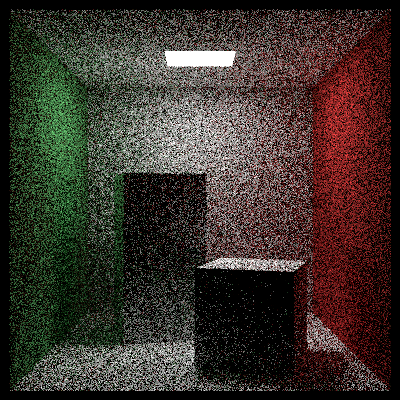
\includegraphics[scale=0.3]{./pic/MC1.png}
	\caption{400*400*50, uniformly scattered}
	\label{fig:label}
\end{figure}

But that is what we are going to improve because now no more rays are sent in important directions. To do this, we need a random direction toward the light--just pick a random point on the light and send a ray in that direction.

\begin{figure}[H]
	\centering
	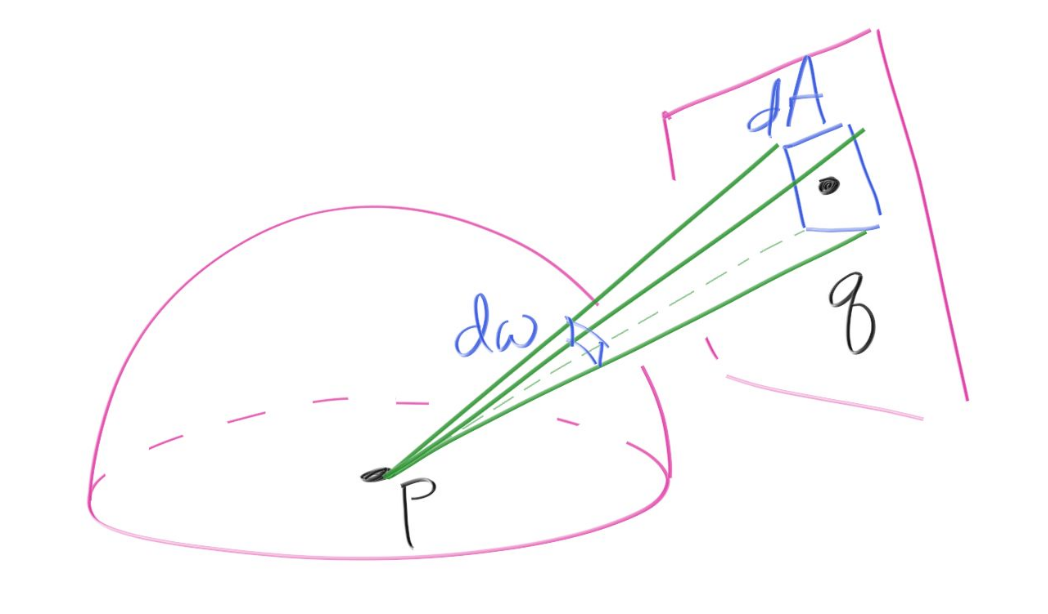
\includegraphics[scale=0.2]{./pic/MC3.png}
	\caption{rays pointing to light}
	\label{fig:label}
\end{figure}

If we are going to sample a point in a little light square with an area of $dA$, the probability should be $dA/A$, and according to the book, the $dw$ should have a geometry relationship with $dA$:
$$
dw = \frac{dA \cdot cos(\alpha)}{distance(p,q)^2}
$$
where $distance(p,q)$ is the distance between the reflecting point and the lighting point, and $\alpha$ is the angle between the light ray and the normal vector of the reflecting surface.



Since sampling in $dw$ should be the same as $dA$, we have
$$
\frac{p(direction)*cos(\alpha)*dA}{distance(p,q)^2} = \frac{dA}{ A}
$$
and we should get:
$$
p(direction) =\frac{distance(p,q)^2} {cos(alpha) *A}
$$

This function means, if we are using such $p(direction)$, we only send scattering light toward the light. This method largely reduce the noise and with only 4 sample in each pixel, we can get a picture as below
	\begin{figure}[H]
	\centering
	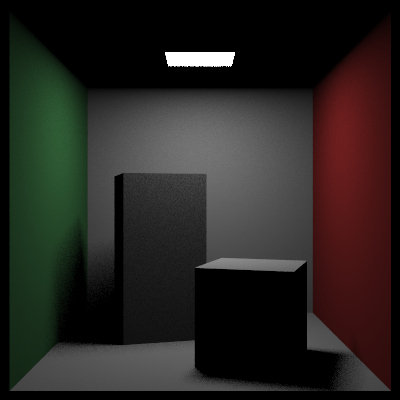
\includegraphics[scale=0.3]{./pic/MC2.png}
	\caption{400*400*50, light source oriented }
	\label{fig:label}
\end{figure}





	\bibliographystyle{IEEEtran}
	\bibliography{IEEEabrv,mylib}
\end{document}
